\documentclass[11pt]{article}
%%%%%%%%% options for the file macros.tex

\def\showauthornotes{1}
\def\showkeys{0}
\def\showdraftbox{0}
% \allowdisplaybreaks[1]


\usepackage{amsmath, ulem, amssymb, amsfonts, hyperref, amsthm, listings, tcolorbox, bbm, xifthen, soul, mathtools}
\usepackage[margin=1in]{geometry}
\usepackage[linesnumbered,lined,boxed,commentsnumbered, ruled]{algorithm2e}
\hypersetup{
    colorlinks=true,
    linkcolor=blue,
    filecolor=magenta,      
    citecolor=magenta,      
    urlcolor=cyan,
}
\usepackage[
    backend=biber,
    style=alphabetic,
    sorting=ynt,
    backref=true
]{biblatex}
\usepackage[shortlabels]{enumitem}
\usepackage{cleveref}

\newtheorem{theorem}{Theorem}[section]
\newtheorem{lemma}[theorem]{Lemma}
\newtheorem{corollary}[theorem]{Corollary}
\newtheorem{claim}[theorem]{Claim}
\newtheorem{fact}[theorem]{Fact}
\newtheorem{open-problem}[theorem]{Open Problem}

\theoremstyle{definition}

\newtheorem{definition}[theorem]{Definition}
\newtheorem{example}[theorem]{Example}

\newtheorem{remark}{Remark}
\newtheorem{question}{Question}

\newcommand{\V}[1]{\mathbf{#1}\ignorespaces}
\renewcommand\AA{\boldsymbol{\mathit{A}}}
\newcommand\LL{\boldsymbol{\mathit{L}}}
\newcommand\MM{\boldsymbol{\mathit{M}}}
\newcommand\II{\boldsymbol{\mathit{I}}}
\newcommand\JJ{\boldsymbol{\mathit{J}}}
\newcommand\KK{\boldsymbol{\mathit{K}}}

\newcommand{\ab}[1]{\langle #1 \rangle}
\renewcommand{\subset}{\subseteq}
\newcommand{\dsquare}{\mathbin{\raisebox{.2ex}{
    \hspace{-.4em}$\bigcirc$\hspace{-.75em}{\rm s}\hspace{.15em}}}}
\newcommand{\from}{\overset{R}{\leftarrow}}
\newcommand{\1}{\mathbbm{1}}

\DeclareMathOperator{\USTCON}{USTCON}
\DeclareMathOperator{\STCON}{STCON}
\allowdisplaybreaks

\usepackage{tikz}
\usepackage[backend=biber]{biblatex}
\addbibresource{papers.bib}
%\usepackage[
%    backend=biber,
% giveninits=true,
% natbib=true,
%    style=alphabetic,
%    url=false, 
 %   doi=true,
%    hyperref,
%    backref=true,
%    backrefstyle=none,
%    maxbibnames=10,
%    sortcites
%]{biblatex}
%\addbibresource{papers.bib}

%%%%%%%%% Authornotes
\newcommand{\Snote}{\Authornote{S}}

% \renewcommand\vec{\V}
\renewcommand\overrightarrow{\vec}
\newcommand\itxt[1]{\intertext{\indent#1}}

\addbibresource{papers.bib}

%%%%%%%%%%%%%%%%%%%%%%%%%

\begin{document}

\newcommand{\coursenum}{{CSC 2240H}}
\newcommand{\coursename}{{Graphs, Matrices, and Optimization}}
\newcommand{\courseprof}{Sushant Sachdeva}

\lecturetitle{}{Solving Laplacians using low-stretch spanning trees}{Ensieh Khazaei, Danya Lette}{23 Dec 2022}

\section{Introduction}

In their 2013 paper ``A Simple, Combinatorial Algorithm for Solving SDD Systems in Nearly-Linear Time" \cite{Kel13}, Kelner et al. proposed an algorithm for getting approximate solutions to SDD systems, that is: systems of the form $A\vec x = \vec b$, in which $A$ is symmetric and diagonally dominant. 

Prior to this work, in 2004, Spielman and Teng proposed their own nearly-linear time Laplacian solver \cite{ST04}. This highly influential work is also highly complex, making it difficult to understand, analyze, and adapt to special cases. The algorithm in \cite{Kel13} is, in contrast, very simple. 

In brief, the algorithm reduces SDD systems to Laplacian systems and, in the context of the electrical networks view of a Laplacian system, aims to find an approximately optimal flow vector by iteratively updating a guess of the network's flow. In each iteration, an edge is sampled from a spanning tree of the network; each edge corresponds to a cycle in the network, and the flow is updated in that iteration by enforcing a conservation of energy law on that cycle. The algorithm runs in $\mathcal O(m \log^2 n \log \log n \log(\epsilon^{-1}))$. 

In these lecture notes, we present the necessary background materials in Section \ref{sec:prelim}, the algorithm itself in Section \ref{sec:algo}. We then discuss the algorithm's correctness and convergence in Section \ref{sec:conv} and, finally, present a geometrical interpretation in Section \ref{sec:geom}.

\section{Preliminaries}\label{sec:prelim}
\subsection{The Problem}
An SDD system is a system of the form $A\vec x = \vec b$, where $A$ is \textit{symmetric} ($A^T = A$) and $A$ is \textit{diagonally dominant} ($\forall i\in[n].A_{ii}\ge\sum_{j\ne i}^{ }|A_{ij}|$). The Kelner paper \cite{Kel13} is aimed at \textbf{approximately} solving an SDD system. In particular, if $A\vec x_{opt} = \vec b$, then $\vec x$ is an approximate solution whenever $$ \|\vec{x} - \vec{x}_{opt}\|_A \le \epsilon \|\vec{x}_{opt}\|_A$$ 

The authors present a reduction from the SDD system $A \vec x = \vec b$ to the Laplacian system $L \vec v = \vec \chi$ satisfying $\sum_ {a \in V} \vec \chi(a)  = 0$, and their subsequent technique pertains to Laplacian solving. In these lecture notes, we omit the reduction and focus on the Laplacian solving, in keeping with the themes of this course. 

If $L^{\dagger} \vec \chi = \vec v _{opt}$, where $L^{\dagger}$ is the Moore-Penrose pseudoinverse of $L$, then an approximate solution $\vec v$ to this Laplacian refers to a vector $\vec v$ satisfying $$\mathbb E\| \vec v - \vec v_{opt}  \|_L \le \sqrt{\epsilon} \| \vec v_{opt} \|_L $$

\subsection{Electrical Networks}

We define electrical network graphs in the usual way. Let $G = (V,E,w)$ be a weighted, connected, undirected graph with $n = |V|$ vertices and $m = |E|$ edges, where edge $e \in E$ has weight $w_e$ and \textit{resistance} $r_e = \frac{1}{w_e}$. Edges  are oriented by the convention that, for the edge incident on $a,b\in V$, one of $(a,b)$ or $(b,a)$ are $\in E$.
Define the incidence matrix $B \in \R^{E \times V}$, the resistance matrix $R \in \R^{E \times E}$, and the Laplacian matrix $L \in \R^{V \times V}$: 
\\ 

\begin{minipage}[b]{0.33333\textwidth}
$$ B_{(a,b),c} = \begin{cases} 1 & a = c \\ -1 & b = c \\ 0 & \text{o.w.}\end{cases}$$
\end{minipage}%
\begin{minipage}[b]{0.33333\textwidth}
$$ R_{e_1,e_2} = \begin{cases} r_e & e = e_1 = e_2 \\ 0 & \text{o.w.} \end{cases}$$
\end{minipage}%
\begin{minipage}[b]{0.33333\textwidth}
$$ L_{a,b} = \begin{cases} \text{wdeg}(a) & a = b \\ -w_{a,b} & \{a,b\} \in E \\ 0 & \text{o.w.}\end{cases}$$
\end{minipage}

\subsection{Electrical Flow and Duality}
\label{section:electrical-flow-duality}
\begin{definition}[Feasible]
A flow $\vec f \in \R^E$ is \textit{feasible} with respect to $\vec \chi \in \R^V$ if $B^T\vec f = \vec \chi $
\end{definition}

For $\vec f \in \R^E$, define its energy as $\xi(\vec f) = \vec f^T R \vec f$. Given a demand vector $\vec \chi$ such that $\sum_{a \in V} \vec \chi(a) = 0$, the \textit{electrical flow problem} is the problem of finding the energy-minimizing feasible flow: 
$$ \vec f_{opt} = \text{argmin}_{\vec f \in \R^E : B^T\vec f = \vec \chi } \xi(\vec f)$$

In the context of electrical networks, a solution to the system $L \vec x = \vec \chi $ concerns a \textit{voltage} vector $\vec x \in \R^V$. However, the algorithm that we will present today searches for a \textit{flow} vector $\vec f \in \R^E$. These two vectors are related via \textit{duality}.  

The electrical flow problem is the Lagrangian dual of solving $L \vec x = \vec \chi$, which finds the energy-maximizing voltage $\vec x$, where, for $\vec v \in \R^V$, voltage energy is defined as $\zeta(\vec v) = 2\vec v \vec \chi - \vec v ^T L \vec v$. 

This is a strong duality, so $\zeta(\vec v_{opt}) = \xi(\vec f_{opt})$. The optimal flow and voltage vectors $\vec f_{opt}$ and $\vec v_{opt}$ satisfy 
$$
\forall (a,b) \in E: \vec f _{opt} ((a,b)) = \frac{\vec v_{opt}(a) - \vec v_{opt}(b)}{r_{(a,b)}}
$$

\begin{definition}[Circulation]
    A flow $\vec f \in \R^E$ is a \textit{circulation} if $B^T\vec f = 0 $
\end{definition}

Kirchoff's Potential Law (KPL) is one form of a conservation of energy law. This law forms the basis for the algorithm. 

\begin{lemma}[KPL]
A feasible flow $\vec f$ is optimal if and only if $\vec f^T R \vec c  = 0$ for all circulations $\vec c \in \R^E$. 
\end{lemma}

\subsection{Low-Stretch Spanning Trees}

A tree is a connected, acyclic, undirected graph. Given a graph $G = (V,E,w)$, a spanning tree $T = (V_T,E_T)$ of $G$ is a tree where $V_T = V$ and $E_T \subseteq E$. We call an edge $e \in E \setminus E_T$ an \textit{off-tree edge}. 

Remark that $E_T \cup \{ e \}$, where $e = (a,b)$ is a off-tree edge, contains exactly one cycle, since there must already be a (unique) path between $a$ and $b$ in $T$. Also note that, for $e, e'$ off-tree edges, if $e 
\ne e'$, the cycle in $E_T \cup \{ e \}$ is distinct from the cycle in $E_T \cup \{ e' \}$, since the former cycle contains $e \not \in E_T$ and latter $e'$. 
\begin{figure}[H]
\begin{minipage}[b]{0.33333\textwidth}
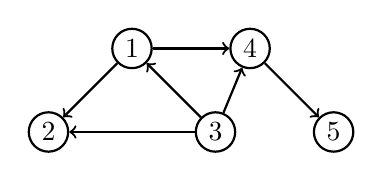
\begin{tikzpicture}[auto,node distance=1.5cm,
        thick,main node/.style={circle,draw,minimum size=0.5cm,inner sep=0pt]}]

    \node[main node] (1) {$1$};
    \node[main node] (2) [below left of=1]  {$2$};
    \node[main node] (3) [below right of=1] {$3$};
    \node[main node] (4) [right of=1] {$4$};
    \node[main node] (5) [right of=3] {$5$};

    \path[->]
    (1) edge node {} (2)
        edge node {} (4)
    (3) edge node {} (1)
        edge node {} (2)
        edge node {} (4)
    (4) edge node {} (5);
\end{tikzpicture}
\\\centering A graph $G = (V, E, w)$. 
\end{minipage}
\begin{minipage}[b]{0.33333\textwidth}
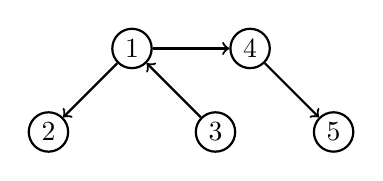
\begin{tikzpicture}[auto,node distance=1.5cm,
        thick,main node/.style={circle,draw,minimum size=0.5cm,inner sep=0pt]}]

    \node[main node] (1) {$1$};
    \node[main node] (2) [below left of=1]  {$2$};
    \node[main node] (3) [below right of=1] {$3$};
    \node[main node] (4) [right of=1] {$4$};
    \node[main node] (5) [right of=3] {$5$};

    \path[->]
    (1) edge node {} (2)
        edge node {} (4)
    (3) edge node {} (1)
    (4) edge node {} (5);
\end{tikzpicture}
\\\centering A spanning tree of $G$. 
\end{minipage}
\begin{minipage}[b]{0.33333\textwidth}
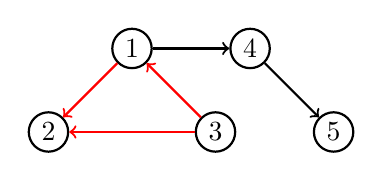
\begin{tikzpicture}[auto,node distance=1.5cm,
        thick,main node/.style={circle,draw,minimum size=0.5cm,inner sep=0pt]}]

    \node[main node] (1) {$1$};
    \node[main node] (2) [below left of=1]  {$2$};
    \node[main node] (3) [below right of=1] {$3$};
    \node[main node] (4) [right of=1] {$4$};
    \node[main node] (5) [right of=3] {$5$};
s
    \path[->]
    (1) edge node {} (4)
    (4) edge node {} (5);
    \path[->, red]
    (3) edge node {} (1)
    (1) edge node {} (2)
    (3) edge node {} (2);
    
\end{tikzpicture}
\\\centering Edge $(3,2)$'s cycle, shown in red. 
\end{minipage}
\caption{An example graph and spanning tree with off-tree edges $(3,2)$ and $(3,4)$}
\label{ex:cycle}
\end{figure}
\begin{definition}(Tree Path)
    For $a,b \in V$, the tree path $P_{(a,b)} \subseteq V \times V$ is the unique path between $a$ and $b$ in $T$.
\end{definition}
\begin{definition}(Tree Cycle)
    For $a,b \in V$, the tree cycle $C_{(a,b)} = \{(a,b)\} \cup P_{(a,b)}$. The vector $\vec c_{(a,b)} \in \R^E$ assigns flow $1$ to each edge $e \in C_{(a,b)}$. 
\end{definition}

\noindent A path $P_e$ corresponds to a vector $\vec p_e$ as follows: for $a,b \in V$, $$\vec p_{e}((a,b)) = \begin{cases} 1 & (a,b) \in P_{e} \cap E \\ -1 & (a,b)  \in P_{e} \land (b,a) \in E  \\ 0 & \text{o.w.} \end{cases}$$

A cycle $C_e$ corresponds to a  vector $\vec c_e$, which is defined analogously to $\vec p_e$. The vector corresponding to a cycle is a circulation, which, recall, means that $B^T \vec c_e = 0$. 


The set of all circulations $\{ \vec c \in \R^E : B^T\vec c = 0\}$ is a subspace called the \textit{cycle space} and the cycles $\{ \vec c_e : e \in E \setminus E_T \}$  determined by the off-tree edges are a basis for this space. 

\begin{example}
    Continuing the example of Figure \ref{ex:cycle}, the cycle basis is $\{ \vec c_{(3,2)}, \vec c_{(3,4)} \}$. The cycle $C'$ with path $\{ (3,2), (2,1), (1,4), (4,3) \}$ and vector $\vec c'$ is not in this basis, but it can be formed from basis elements.
    \begin{figure}[H]
    \begin{minipage}{0.48\textwidth}
    \centering 
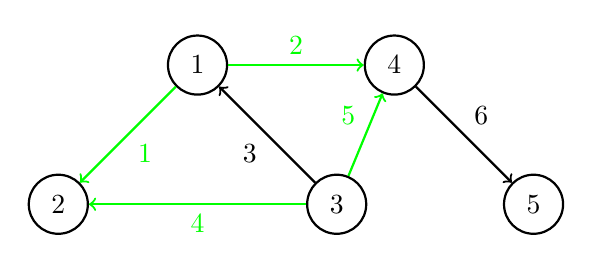
\begin{tikzpicture}[auto,node distance=2.5cm,
        thick,main node/.style={circle,draw,minimum size=0.75cm,inner sep=0pt]}]

    \node[main node] (1) {$1$};
    \node[main node] (2) [below left of=1]  {$2$};
    \node[main node] (3) [below right of=1] {$3$};
    \node[main node] (4) [right of=1] {$4$};
    \node[main node] (5) [right of=3] {$5$};

    \path[->]
    (3) edge node {3} (1)
    (4) edge node {6} (5);
    \path[->, green]
    (1) edge node {1} (2)
        edge node {2} (4)
    (3) edge node {4} (2)
    (3) edge node {5} (4);
\end{tikzpicture}
\\\centering 
\end{minipage}
\begin{minipage}{0.48\textwidth}
\vspace{-10px}
    $$\textcolor{red}{\vec c_{(3,2)}} = 
    \textcolor{red}{
    \begin{bmatrix}
        -1 \\ 0 \\ -1 \\ 1 \\ 0 \\ 0 
    \end{bmatrix}}, \vec c_{(3,4)} = \begin{bmatrix}
        0 \\ -1 \\ -1 \\ 0 \\ 1 \\ 0 
    \end{bmatrix},
    \textcolor{green}{\vec c'} = \textcolor{green}{\begin{bmatrix}
        -1 \\ 1 \\ 0 \\ 1 \\ -1 \\ 0 
    \end{bmatrix}} = \textcolor{red}{\vec c_{(3,2)}} - \vec c_{(3,4)}
    $$
\end{minipage}
\caption{The composite cycle $C'$, shown in green, is comprised of  basis cycles. }
\end{figure}
\end{example}

A given graph may have several spanning trees, some of which result in faster convergence of the algorithm than others. We quantify the desirability of a spanning tree according to its \textit{condition number}. This number represents how well the resistances of off-tree edges are approximated by the resistance along the cycle determined by that edge. 
\begin{definition}[Cycle Resistance $R_e$]$R_e = \sum_{e' \in C_e} r_{e'} = \vec c_e^T R \vec c_e$
\end{definition}
\begin{definition}[Tree Condition Number $\tau$]
    $\tau(T) = \sum_{e\ in E \setminus E_T} \frac{R_e}{r_e}$. 
\end{definition}
\begin{definition}[Stretch $st$] For $e \in E$, $st(e) = \frac{\sum_{e' \in P_e} r_{e'}}{r_e}$ and $st(T) = \sum_{e \in E} st(e)$.
\\
\\
We remark that $\tau(T) =  st(T) + m - 2n + 2 $; so, a low-stretch tree has a low condition number. Other works have yielded useful techniques for producing low-stretch spanning trees. 

\begin{theorem}[\cite{AN12}] 
\label{thm:AN12}
    In $\mathcal O(m \log n \log \log n)$ time we can compute a spanning tree $T$ with a total stretch $st(T) = O(m \log n \log \log n)$. 
\end{theorem}
    
\end{definition}



% Generally speaking, given an inner product $\langle ., . \rangle$, the orthogonal projection of $x$ along $y$ (resp. $y^\perp$) in that inner product space is $Proj_y(x) = \frac{\langle y, x \rangle }{ \langle y , y\rangle}y$ (resp. $Proj_{y^\perp}(x) = x - \frac{\langle y, x \rangle}{ \langle y , y\rangle}y$). Noting that $\langle \vec a , \vec b \rangle = \vec a^T R\vec b$ is an inner product, denote $S$ this inner product space. Since $\| \vec a \|^2_R = \langle \vec a, \vec a \rangle$, we can see that the above expression $\vec f_i - \frac{\vec f_i^T R \vec c_{e_i}  }{\| \vec c_{e_i}\|^2_R} c_{e_i}$ is an orthogonal projection of $\vec f_i$ along $\vec c_{e_i}^\perp$ in $S$, in the ordinary sense of projection, meaning that this projection operator $\Pi_{e_i}$ is symmetric and idempotent. 

\section{The Algorithm}\label{sec:algo}

In this section, we present a simple version of the algorithm presented in \cite{Kel13}, called \texttt{SimpleSolver}. 

\begin{figure}[H]
\centering 
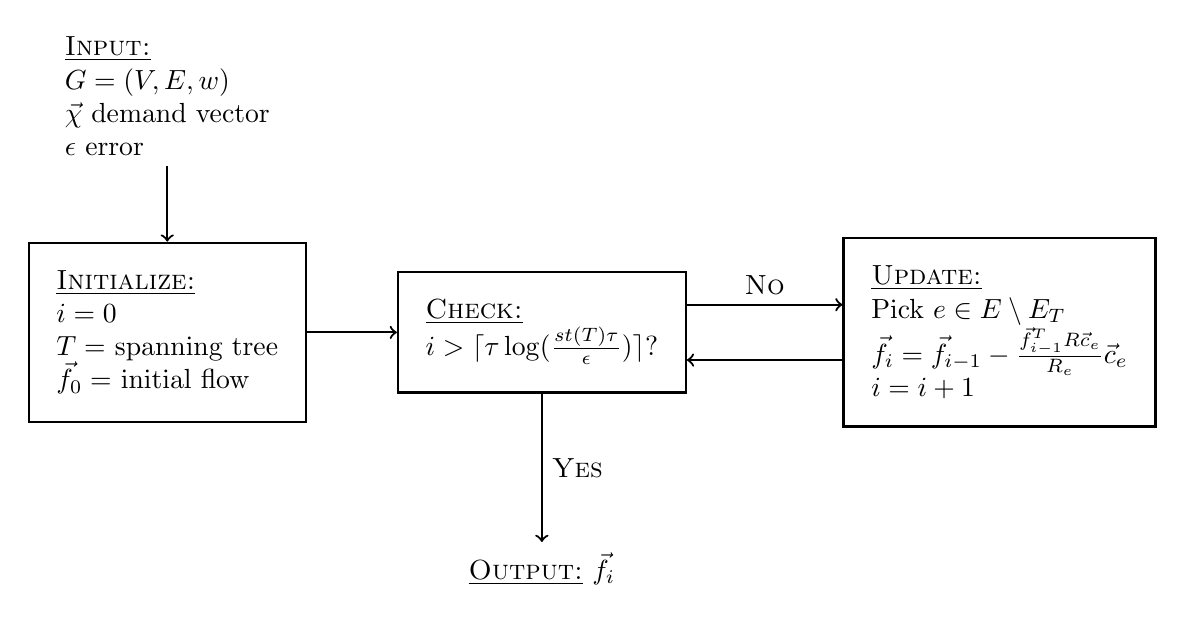
\begin{tikzpicture}[auto,node distance=3cm,align=left,
        thick,main node/.style={rectangle,draw,minimum size=1cm,inner sep=10pt]}]

    \node[] (1) {\underline{\textsc{Input:}}\\$G = (V,E,w)$\\ $\vec \chi$ demand vector \\ $\epsilon$ error};
    \node[main node] (2) [below of = 1]  {\underline{\textsc{Initialize:}}\\$i = 0$\\ $T = $ spanning tree \\$\vec f_0 = $ initial flow };
    \node[main node] (3) [xshift=5em, right of =2] {\underline{\textsc{Check:}}\\$i > \lceil \tau \log(\frac{st(T) \tau}{\epsilon} ) \rceil $?};
    \node[main node] (5) [xshift=8em, right of =3] {\underline{\textsc{Update:}} \\Pick $e \in E \setminus E_T$ \\$\vec f_i = \vec f_{i-1} - \frac{\vec f_{i-1}^T R \vec c_e}{R_e} \vec c_e $ \\ $i = i + 1$};
    \node[] (6) [below of=3] {\underline{\textsc{Output:}} $\vec f_i$};

    \path[->]
    (1) edge node {} (2)
    (2) edge node {} (3)
    (3) edge node {\textsc{Yes}} (6)
    (3) edge [transform canvas={yshift=1em}] node {\textsc{No}} (5)
    (5) edge  [transform canvas={yshift=-1em}] node {} (3);
\end{tikzpicture}
\caption{An outline of the \texttt{SimpleSolver} algorithm of \cite{Kel13} }
\end{figure}

\subsection{Initialization}
From Theorem \ref{thm:AN12}, the algorithm starts by choosing a spanning tree with stretch in $\mathcal O(m \log n \log \log n)$ in time $\mathcal O(m \log n \log \log n)$. 

An initial flow $\vec f_0$ is computed; this flow should be feasible, that is, satisfy $B^T\vec f = \vec \chi$. A feasible flow may be found in $\mathcal O(m + n)$ using Depth-First Search (DFS). Recalling that $\sum_{a \in V} \vec\chi (a) = 0$, we can make the reasonable simplifying assumption that, for some $s, t \in V$, $\vec \chi =  \textbf{1}_s - \textbf{1}_t$. $P_{(s,t)} \subseteq V \times V$ is the path between $s$ and $t$ in $T$. Now consider the flow $\vec f_0$ defined as $$ \vec f_0(a) = \begin{cases}
    1 & a \in P_{(s,t)} \\ 0 & \text{o.w.}
\end{cases}$$
By definition of the incidence matrix $B$, for each edge $e = (a,b) \in E$, the $e$th row of $B$ is $\textbf 1_{a}^T - \textbf 1_{b}^T$. So,  $$B^T \vec f_0 = \sum_{(a,b) \in P_{(s,t)}} \textbf 1_{a} - \textbf 1_{b} = \vec \chi,$$. which is feasible. So, a feasible initial flow $\vec f_0$ is computed in linear time using DFS. 

\subsection{Cycle Update}
\label{algorith:cycle-update}
In order to choose a cycle in the cycle basis, an edge is selected from $E \setminus E_T$. These edges are sampled with probability distribution $P(e) = \frac{1}{\tau(T)} \cdot \frac{R_e}{r_e}$. Once an edge $e$ is selected, the current flow $\vec f_{i-1}$ is updated:
$$\vec f_i = \vec f_{i-1} - \frac{\vec f_{i-1}^TR\vec c_e}{R_e}\vec c_e$$

The new flow satisfies KPL on the cycle $C_e$, that is: $\vec f_i^T R \vec c_e = 0$, since $\vec c_e^TR\vec c_e = R_e$. In addition, because $\vec c_e$ is a circulation, $B^T \vec c_e = 0$, which implies that the new flow is feasible, meaning $B^T \vec f_i = \vec \chi$. 

\subsection{Runtime}

Initialization runs in $\mathcal O(m \log n \log \log n)$. Cycle updates, which are repeated $\lceil \tau \log (\frac{st(T) \tau}{\epsilon}) \rceil$ times, can be performed in $\mathcal O(\log n)$, using a data structure presented in \cite{Kel13} which is out of scope of these lecture notes. In all, algorithm runs in $\mathcal O (m \log^2 n \log{ \log n \log{(\epsilon^{{-1}})}})$. 

% \begin{algorithm}
% \SetAlgoLined
% \SetKwInOut{Input}{Input}
% \SetKwInOut{Output}{Output}
% \Input{$G = (V, E, r)$, $\boundary \in \rvertvec$, $\epsilon \in \rPos$}
% \Output{$\flow \in \redgevec$ and $\volt \in \rvertvec$}
% \BlankLine
% \ \ $T := $ low-stretch spanning tree of $G$\;\\
% $\flow_0 := $ unique flow on $T$ such that $\incMatrix^T \flow_0 = \boundary$\;\\
% $\edgeSampleProb{e} := \frac{1}{\treeCondition(\tree)} \cdot \frac{\cycleResistance{e}}{r_e}$ for all
% $e \in \offtreeEdgeSet$ \;\\
% $\nIter = \big\lceil\treeCondition \log \big(\frac{\stretchTotal{\tree}
%     \cdot \treeCondition(\tree)}{\epsilon}\big)\big\rceil$\;\\
% \For{$i = 1$ to $\nIter$}
% {
%     Pick random $e_i \in \offtreeEdgeSet$ by probability distribution
%     $\sampleProbVec$ \;\\ 
%     $\flow_i = \flow_{i - 1} - \frac{\cyclePotential{e}{\flow_{i - 1}}}
%         {\cycleResistance{e}}
%     \treeCycleVec{e}$ \;
% }
% \Return{$\flow_{\nIter}$ and its tree induced voltages $\volt_{\nIter}$}
% \caption{\label{algm:simplealgorithm}$\simpleSolver$}
% \end{algorithm}

\section{Convergence Analysis}\label{sec:conv}
In this section we analyze the convergence rate of \texttt{SimpleSolver} algorithm. In other words, we investigate whether this algorithm can converge to the optimal solution after finite iterations or not. For this purpose, we should show that after finite iterations, the algorithm's solution approach to the optimal solution with ratio $\epsilon$ or mathematically, the following equation should be satisfied. \\
For $\forall ~~ 0<\epsilon<1, \exists ~ i$ that the Equation \ref{eq:convergence} is satisfied.
\begin{equation}
    \label{eq:convergence}
    \| X_i -X^* \|_2 \leq \epsilon \|X_0 - X^* \|_2
\end{equation}
where $X_i$ and $X_0$ are the algorithm's solution in the $i$-th and first iterations, respectively. $\epsilon$ is lower than 1, but our desired value is very close to zero like 0.001 or $10^{-5}$. When we can find an $i$ such that the Equation \ref{eq:convergence} is established in that iteration, then we can conclude the algorithm can converge to the optimal solution with ratio $\epsilon$.
Theorem \ref{thrm:convergence} is equivalent to Equation \ref{eq:convergence} in the context of \texttt{SimpleSolver} algorithm.

\begin{theorem}
    Each iteration $i$ of \texttt{SimpleSolver} computes feasible $\overrightarrow{f}_i \in \mathds{R}^E$ such that
    \begin{center}
        $\mathds{E}[\xi_r(\overrightarrow{f}_i)]-\xi_r(\overrightarrow{f}_{opt}) \leq (1-\frac{1}{\tau})^i (\xi_r(\overrightarrow{f}_0) - \xi_r(\overrightarrow{f}_{opt}))$ 
    \end{center}
    \label{thrm:convergence}
\end{theorem}
where $\xi_r(\overrightarrow{f}_i)$, $\xi_r(\overrightarrow{f}_{opt})$, and $\xi_r(\overrightarrow{f}_0)$ are the energy of $i$-th iteration, optimal energy, and energy of primary current flow, respectively. $\tau$ is the condition number of spanning tree of $T$ which is fixed in all iterations and it is positive. Therefore, $(1-\frac{1}{\tau})$ would be lower than 1 and as $i$ grows, the value of $(1-\frac{1}{\tau})^i$ becomes closer to zero. The proof of Theorem \ref{thrm:convergence} is divided into three steps. In Section \ref{cycle-update-progress}, we analyze the energy gain of a single algorithm iteration, in Section \ref{distance-to-optimality}, we bound the distance to optimality in a single algorithm iteration, and in Section \ref{section:convergence-proof}, we connect these to prove the theorem.

\subsection{Cycle Update Progress}
\label{cycle-update-progress}
In Section \ref{algorith:cycle-update}, we observed that the current flow vector in each iteration is updated with 

$-\frac{\Delta_{c_e}(\overrightarrow{f}_i)}{R_e} \overrightarrow{c}_e$ vector, where $\Delta_{c_e}(\overrightarrow{f}_i) = \overrightarrow{f}_i^\top \mathbf{R} \overrightarrow{c}_e$ and $R_e=\overrightarrow{c}_e^\top \mathbf{R} \overrightarrow{c}_e$. In this section, from a mathematical perspective, we investigate why this update vector approaches the algorithm to the optimal solution.\\
The first idea that comes to our mind when we want to calculate the optimal update value is derivation. Therefore, we consider the $\xi_r(\overrightarrow{f}+\alpha \overrightarrow{c})$ and find the best $\alpha$ that can minimize the energy.
\begin{center}
    
    $\frac{\partial \xi_r(\overrightarrow{f}+\alpha \overrightarrow{c})}{\partial \alpha} =
    \frac{\partial (\overrightarrow{f}+\alpha \overrightarrow{c})^\top \textbf{R} (\overrightarrow{f}+\alpha \overrightarrow{c})}{\partial \alpha}= 2 \overrightarrow{f} \textbf{R} \overrightarrow{c} + 2 \alpha \overrightarrow{c}^\top \textbf{R} \overrightarrow{c}$
\end{center}
\begin{equation}
    \label{gradient-to-alpha}
    2 \overrightarrow{f} \textbf{R} \overrightarrow{c} + 2 \alpha \overrightarrow{c}^\top \textbf{R} \overrightarrow{c}=0 \implies \alpha^* = -\frac{\overrightarrow{f} \textbf{R} \overrightarrow{c}}{\overrightarrow{c}^\top \textbf{R} \overrightarrow{c}}
\end{equation}
In the second stage, we verify whether this $\alpha^*$ can decrease the energy of the electrical network in each iteration or not. Therefore, we calculate the energy difference between two sequential iterations by substitution of $\alpha^*$. 
\begin{center}
    $\xi_r(\overrightarrow{f}+\alpha^* \overrightarrow{c}) - \xi_r(\overrightarrow{f})=(\overrightarrow{f}+\alpha^* \overrightarrow{c})^\top \textbf{R} (\overrightarrow{f}+\alpha^* \overrightarrow{c}) - \overrightarrow{f}^\top \textbf{R} \overrightarrow{f}=$
\end{center}
\begin{equation}
\label{energy-decrease}
    {\alpha^*}^2 \overrightarrow{c} \textbf{R} \overrightarrow{c}+2 \alpha^* \overrightarrow{f}^\top \textbf{R} \overrightarrow{c}=-\frac{(\overrightarrow{f}^\top \mathbf{R} \overrightarrow{c})^2}{\overrightarrow{c}^\top \mathbf{R} \overrightarrow{c}}
\end{equation}
According to Equation \ref{energy-decrease}, it can be seen the energy in two sequential iterations decreases if we update the flow vector with the corresponding $\alpha$.
We summarize the update value and energy decrease in Lemma \ref{energy-improvement}.
\begin{lemma}
    \label{energy-improvement}
    For $\overrightarrow{f} \in \mathds{R}^E$, $\overrightarrow{c} \in \mathds{R}^E$, and $\alpha^*=-\frac{\overrightarrow{f} \mathbf{R} \overrightarrow{c}}{\overrightarrow{c}^\top \mathbf{R} \overrightarrow{c}} \in \mathds{R}$ we have
    \begin{center}
        $argmin_{\alpha \in \mathds{R}}~ \xi_r(\overrightarrow{f}+\alpha \overrightarrow{c})=-\frac{\overrightarrow{f} \mathbf{R} \overrightarrow{c}}{\overrightarrow{c}^\top \mathbf{R} \overrightarrow{c}} \text{~~~~~ and ~~~~~}\xi_r(\overrightarrow{f}+\alpha^* \overrightarrow{c}) - \xi_r(\overrightarrow{f})=-\frac{(\overrightarrow{f}^\top \mathbf{R} \overrightarrow{c})^2}{\overrightarrow{c}^\top \mathbf{R} \overrightarrow{c}}$
    \end{center}
\end{lemma}
If we define $\overrightarrow{c}=\overrightarrow{c}_e$ is a tree cycle for some off-tree edge $e \in E \setminus T$, since $R_e= \overrightarrow{c}_e^\top \mathbf{R} \overrightarrow{c}_e$ and $\Delta_{c_e}(\overrightarrow{f})=\overrightarrow{f}^\top \mathbf{R} \overrightarrow{c}_e$, this procedure is precisely the iterative step of \texttt{SimpleSolver}, i.e. a cycle update. Lemma \ref{lemma:cycle-update} states the energy decrease of a cycle update is exactly the energy of a resistor with resistance $R_e$ and potential drop $\Delta_{c_e}(\overrightarrow{f})$.
\begin{lemma}
    \label{lemma:cycle-update}
    For feasible $\overrightarrow{f} \in \mathds{R}^E$ and $e \in E \setminus T$ we have
    \begin{center}
        $\xi_r(\overrightarrow{f}-\frac{\Delta_{c_e}(\overrightarrow{f})}{R_e} \overrightarrow{c}_e) - \xi_r(\overrightarrow{f})=-\frac{\Delta_{c_e}(\overrightarrow{f})^2}{R_e}$
    \end{center}
\end{lemma}

\subsection{Distance to Optimality}
\label{distance-to-optimality}
In this section, we calculate the gap between $\overrightarrow{f}$ and $\overrightarrow{v}$ in the dual problem. Since the energy function of $\overrightarrow{f}$ is convex and Slater's condition is satisfied, the duality gap between the primal and dual problems is zero. Figure \ref{fig:duality-gap} shows the gap between the primal and dual problems. 
\begin{center}
\begin{figure}[!ht]
\begin{tikzpicture}
    \node[anchor=south west,inner sep=0] at (5.0,0.0) {\includegraphics[scale=0.5]{Images/Convergence/dual_problem.drawio.png}};
    \draw (4.8,1.5) node {$\xi_r(\overrightarrow{v}_i)$};
    \draw (7.1,0.7) node {$\xi_r(\overrightarrow{v})$};
    \draw (7.1,5.9) node {$\xi_r(\overrightarrow{f})$};
    \draw (4.8,5.5) node {$\xi_r(\overrightarrow{f}_i)$};
    \draw (3.5,3.2) node {$\xi_r(\overrightarrow{f}_{opt})=\xi_r(\overrightarrow{v}_{opt})$};
    \draw (12.2,3.4) node {$gap(\overrightarrow{f}_i, \overrightarrow{v}_i)$};
\end{tikzpicture}
\caption{Visualization for primal and dual functions in electrical network energy} 
\label{fig:duality-gap}
\end{figure}
\end{center}
Figure \ref{fig:duality-gap} makes smoother understanding the distance between $\overrightarrow{f}$, $\overrightarrow{f}_{opt}$, $\overrightarrow{v}$, and $\overrightarrow{v}_{opt}$. Here we derive a simple expression for the duality gap between $\overrightarrow{f}$ and its tree-induced voltages $\overrightarrow{v}$ in terms of cycle potentials. Lemma \ref{lemma:tree-gap} states this quantity in terms of cycle potentials.
\begin{lemma}
    \label{lemma:tree-gap}
    For feasible $\overrightarrow{f} \in \mathds{R}^E$ and tree induced voltages $\overrightarrow{v} \in \mathds{R}^V$ we have
    \begin{center}
        $gap(\overrightarrow{f},\overrightarrow{v})=\sum_{e \in E \setminus T} \frac{\Delta_{c_e}(\overrightarrow{f})^2}{r_e}$
    \end{center}
\end{lemma}
\textit{Proof.} We defined the primal and dual energy in Section \ref{section:electrical-flow-duality}, therefore, we have
\begin{equation}
    \label{eq:gap-definition}
    gap(\overrightarrow{f},\overrightarrow{v})=\overrightarrow{f}^\top \mathbf{R} \overrightarrow{f} - (2 \overrightarrow{v}^\top \overrightarrow{\chi} - \overrightarrow{v}^\top \mathbf{L} \overrightarrow{v})
\end{equation}
If we substitute $\mathbf{B}^\top \overrightarrow{f} = \overrightarrow{\chi}$ and $\mathbf{L}=\mathbf{B}^\top \mathbf{R}^{-1} \mathbf{B}$ in Equation \ref{eq:gap-definition}, we get
\begin{center}
    $gap(\overrightarrow{f},\overrightarrow{v})=\overrightarrow{f}^\top \mathbf{R} \overrightarrow{f} - 2 \overrightarrow{v}^\top \mathbf{B}^\top \overrightarrow{f} + \overrightarrow{v}^\top \mathbf{B}^\top \mathbf{R}^{-1} \mathbf{B} \overrightarrow{v})=(\mathbf{R}\overrightarrow{f}-\mathbf{B}\overrightarrow{v})^\top \mathbf{R}^{-1} (\mathbf{R}\overrightarrow{f}-\mathbf{B}\overrightarrow{v})$
\end{center}
\begin{equation}
    =\sum_{e \in E } \frac{1}{r_e}(\overrightarrow{f}(e)r_e - \Delta_{\overrightarrow{v}}(e))^2
\end{equation}
In this stage, we used the definition of tree voltages in Equation \ref{eq:tree-voltages} to simplify $gap(\overrightarrow{f}, \overrightarrow{v})$.
\begin{equation}
    \label{eq:tree-voltages}
    \forall~ a,b \in V ~~:~~ \Delta_{\overrightarrow{v}}(a,b)=\overrightarrow{v}(a) - \overrightarrow{v} (b) = \sum_{e \in P_{as}} \overrightarrow{f}(e) r_e + \sum_{e \in P_{sb}} \overrightarrow{f}(e) r_e = \sum_{e \in P_{ab}} \overrightarrow{f}(e) r_e
\end{equation}
We know that 
\begin{equation}
    \label{eq:tree-voltages-cases}
    \overrightarrow{f}(e) r_e - \Delta_{\overrightarrow{v}}(e) = \begin{cases}
        0 &  \forall ~ e \in T \\
        \Delta_{c_e}(\overrightarrow{f})  &  \forall ~ e \in E \setminus T 
\end{cases}
\end{equation}
is satisfied during the algorithm. Figure \ref{fig:voltage-difference} shows an electrical network to smooth understanding of Equation \ref{eq:tree-voltages-cases}.
\begin{figure}[!h]
    \centering
    \includegraphics[scale=0.44]{Images/Convergence/voltage_difference.jpg}
    \caption{An example of an electrical network with induced current 1A between nodes $b$ and $c$ (the resistance of all edges is equal to $1 \Omega$)}
    \label{fig:voltage-difference}
\end{figure} \\
1A current is induced between nodes $b$ and $c$ in the electrical network in Figure \ref{fig:voltage-difference}. Assume one edge from the spanning tree, which is shown with red edges in the graph, like edge $(c,a)$, and investigate the relation $\overrightarrow{f}(e)r_e - \Delta_{\overrightarrow{v}}(e)$ in it (the resistance of all edges in the network is equal to $1 \Omega$)). 
\begin{center}
    $\overrightarrow{f}((c,a))r_{(c,a)} = (1 A) \times (1 \Omega)=1v$\\
    ~\\
    $\Delta_{\overrightarrow{v}}(c,a)=\overrightarrow{v}(c) - \overrightarrow{v} (a) = \sum_{e \in P_{cs}} \overrightarrow{f}(e) r_e + \sum_{e \in P_{sa}} \overrightarrow{f}(e) r_e $\\
    $= [\overrightarrow{f}((e,s))r_{(e,s)} + \overrightarrow{f}((a,e))r_{(a,e)} + \overrightarrow{f}((c,a))r_{(c,a)}]-[\overrightarrow{f}((e,s))r_{(e,s)} + \overrightarrow{f}((a,e))r_{(a,e)}]$\\
    $=\overrightarrow{f}((c,a))r_{(c,a)}=(1 A) \times (1 \Omega)=1v$\\
    ~\\
    $\implies \overrightarrow{f}((c,a))r_{(c,a)} - \Delta_{\overrightarrow{v}}(c,a)=0$
\end{center}
Now, consider an edge outside of the spanning tree such as $(e,f)$ and investigate the relation $\overrightarrow{f}(e)r_e - \Delta_{\overrightarrow{v}}(e)$ for this edge.
\begin{center}
    $\overrightarrow{f}((e,f))r_{(e,f)} = (0 A) \times (1 \Omega)=0v$\\
    ~\\
    $\Delta_{\overrightarrow{v}}(e,f)=\overrightarrow{v}(e) - \overrightarrow{v} (f) = \sum_{e \in P_{es}} \overrightarrow{f}(e) r_e + \sum_{e \in P_{sf}} \overrightarrow{f}(e) r_e $\\
    $= [\overrightarrow{f}((e,s))r_{(e,s)}]-[\overrightarrow{f}((e,s))r_{(e,s)} + \overrightarrow{f}((a,e))r_{(a,e)} + \overrightarrow{f}((b,a))r_{(b,a)}+ \overrightarrow{f}((f,b))r_{(f,b)}]$\\
    $=-\overrightarrow{f}((a,e))r_{(a,e)} - \overrightarrow{f}((b,a))r_{(b,a)} - \overrightarrow{f}((f,b))r_{(f,b)}$\\
    $=-(0 A) \times (1 \Omega) -(1 A) \times (1 \Omega) -(0 A) \times (1 \Omega)=-1v$\\
    ~\\
    $\implies \overrightarrow{f}((e,f))r_{(e,f)} - \Delta_{\overrightarrow{v}}(e,f)=$\\
    $\overrightarrow{f}((a,e))r_{(a,e)} + \overrightarrow{f}((b,a))r_{(b,a)} + \overrightarrow{f}((f,b))r_{(f,b)}$\\
    $=\sum{e \in P_{ef}}\overrightarrow{f}(e)r_e=\Delta_{c_{(e,f)}}(\overrightarrow{f})$
\end{center}
We showed the correctness of Equation \ref{eq:tree-voltages-cases} with an electrical network example. Therefore, if we substitute Equation \ref{eq:tree-voltages-cases} in the simplified definition of $gap(\overrightarrow{f}, \overrightarrow{v})$
\begin{center}
    $gap(\overrightarrow{f}, \overrightarrow{v})=\sum_{e \in E } \frac{1}{r_e}(\overrightarrow{f}(e)r_e - \Delta_{\overrightarrow{v}}(e))^2$\\
    $=\sum_{e \in T } \frac{1}{r_e}(\overrightarrow{f}(e)r_e - \Delta_{\overrightarrow{v}}(e))^2 + \sum_{e \in E \setminus T } \frac{1}{r_e}(\overrightarrow{f}(e)r_e - \Delta_{\overrightarrow{v}}(e))^2$\\
    $=0+\sum_{e \in E \setminus T} \frac{1}{r_e}\Delta_{c_e}(\overrightarrow{f})^2=\sum_{e \in E \setminus T} \frac{1}{r_e}\Delta_{c_e}(\overrightarrow{f})^2$
\end{center}
The proof in this step is complete and Lemma \ref{lemma:tree-gap} is proved for each electrical network. $\square$

\subsection{Convergence Proof}
\label{section:convergence-proof}
In this section, we find an interpretation of energy decrease in two sequential iterations according to the duality gap in order to bound the convergence of \texttt{SimpleSolver} algorithm.\\
In the first step, we state the expectation of energy decrease in two sequential iterations in Lemma \ref{lemma:expected-progress}.
\begin{lemma}
    \label{lemma:expected-progress}
    For iteration $i$ of \texttt{SimpleSolver} algorithm, we have
    \begin{center}
    $\mathds{E}[\xi_r(\overrightarrow{f}_i)-\xi_r(\overrightarrow{f}_{i-1})|~gap(\overrightarrow{f}_{i-1}, \overrightarrow{v}_{i-1})]=-\frac{gap(\overrightarrow{f}_{i-1}, \overrightarrow{v}_{i-1})}{\tau}$
    \end{center}
\end{lemma}
\textit{Proof.} In each iteration $i$, \texttt{SimpleSolver} algorithm picks a random $e_i \in E \setminus T$ with probability $p_{e_i}$. Therefore, we can calculate the expectation as follows.
\begin{equation}
    \label{eq:energy-decrease-expectation}
    \mathds{E}[\xi_r(\overrightarrow{f}_i)-\xi_r(\overrightarrow{f}_{i-1})|~gap(\overrightarrow{f}_{i-1}, \overrightarrow{v}_{i-1})]=\sum_{e \in E} p_e [\xi_r(\overrightarrow{f}_i)-\xi_r(\overrightarrow{f}_{i-1})]
\end{equation}
According to the \texttt{SimpleSolver} algorithm, $p_e=\frac{1}{\tau}\frac{R_e}{r_e}$ and using Lemma \ref{lemma:cycle-update}, the energy decreas between two sequential iterations for $\forall~e \in E \setminus T$ is equal to $-\frac{\Delta_{c_e}(\overrightarrow{f})^2}{R_e}$ and it is zero for edges on spanning tree. By substitution of these quantities in Equation \ref{eq:energy-decrease-expectation}, we get
\begin{center}
    
    $\mathds{E}[\xi_r(\overrightarrow{f}_i)-\xi_r(\overrightarrow{f}_{i-1})|~gap(\overrightarrow{f}_{i-1}, \overrightarrow{v}_{i-1})]=\sum_{e \in E} p_e [\xi_r(\overrightarrow{f}_i)-\xi_r(\overrightarrow{f}_{i-1})]$
\end{center}
\begin{equation}
    \label{eq:simplified-energy-decrease-expectation}
    =\sum_{e \in E\setminus T} \frac{1}{\tau}\frac{R_e}{r_e} (-\frac{\Delta_{c_e}(\overrightarrow{f}_{i-1})^2}{R_e})
\end{equation}
In Lemma \ref{lemma:tree-gap}, we observed that $\sum_{e \in E \setminus T} \frac{\Delta_{c_e}(\overrightarrow{f})^2}{r_e}=gap(\overrightarrow{f},\overrightarrow{v})$. By using Lemma \ref{lemma:tree-gap}, Equation \ref{eq:simplified-energy-decrease-expectation} can be simplified as follows.
\begin{center}
    $\mathds{E}[\xi_r(\overrightarrow{f}_i)-\xi_r(\overrightarrow{f}_{i-1})|~gap(\overrightarrow{f}_{i-1}, \overrightarrow{v}_{i-1})]=\sum_{e \in E\setminus T} \frac{1}{\tau}\frac{R_e}{r_e} (-\frac{\Delta_{c_e}(\overrightarrow{f}_{i-1})^2}{R_e})$\\
    $=-\frac{1}{\tau} \sum_{e \in E\setminus T} \frac{\Delta_{c_e}(\overrightarrow{f}_{i-1})^2}{r_e})=-\frac{gap(\overrightarrow{f}_{i-1}, \overrightarrow{v}_{i-1})}{\tau}$
\end{center}
Hence, the proof of Lemma \ref{lemma:expected-progress} is finished. $\square$ \\
Next, we try to show that each iteration decreases the expected energy difference between the current flow and the optimal flow by a ratio $(1-\frac{1}{\tau})$. Lemma \ref{lemma:convergence-rate} expresses this.
\begin{lemma}
    \label{lemma:convergence-rate}
    For all $i \geq 0$, we define a random variable $D_i \stackrel{\text{def}}{=} \xi_r(\overrightarrow{f}_i)-\xi_r(\overrightarrow{f}_{opt})$. Then for all iterations $i \geq 1$, we have
    \begin{center}
        $\mathds{E}[D_i] \leq (1-\frac{1}{\tau}) \mathds{E}[D_{i-1}]$
    \end{center}
\end{lemma}
\textit{Proof.} Since in each iteration of \texttt{SimpleSolver}, one of a finite number of edges is chosen, clearly, $D_i$ is a discrete random variable and by the law of total expectation we have
\begin{equation}
    \label{eq:D-expectation}
    \mathds{E}[D_i]=\sum_{e} \mathds{E}[D_i|D_{i-1}=c]Pr[D_{i-1}=c]
\end{equation}
We try to simplify $\mathds{E}[D_i|D_{i-1}=c]$.
\begin{center}
    
    $\mathds{E}[D_i|D_{i-1}=c] = \mathds{E}[\xi_r(\overrightarrow{f}_i)-\xi_r(\overrightarrow{f}_{opt})|D_{i-1}=c]$\\
    $= \mathds{E}[(\xi_r(\overrightarrow{f}_i) - \xi_r(\overrightarrow{f}_{i-1}))+(\xi_r(\overrightarrow{f}_{i-1}) - \xi_r(\overrightarrow{f}_{opt}))|D_{i-1}=c] $\\
    $= \mathds{E}[(\xi_r(\overrightarrow{f}_i) - \xi_r(\overrightarrow{f}_{i-1}))+D_{i-1}|D_{i-1}=c] $
\end{center}
\begin{equation}
    \label{eq:conditional-expectation-D}
    = c + \mathds{E}[(\xi_r(\overrightarrow{f}_i) - \xi_r(\overrightarrow{f}_{i-1}))|D_{i-1}=c]
\end{equation}
From Figure \ref{fig:duality-gap}, it can be easily observed that $D_{i-1} \leq gap(\overrightarrow{f}_{i-1},\overrightarrow{v}_{i-1})$ is always satisfied. Using this fact and Lemma \ref{lemma:expected-progress}, we will have
\begin{equation}
    \label{eq:conditional-expectation-D-gap}
    \mathds{E}[(\xi_r(\overrightarrow{f}_i) - \xi_r(\overrightarrow{f}_{i-1}))|D_{i-1}=c]=-\frac{gap(\overrightarrow{f}_{i-1}, \overrightarrow{v}_{i-1})}{\tau} \leq -\frac{D_{i-1}}{\tau}=-\frac{c}{\tau}
\end{equation}
By substitution of Equation \ref{eq:conditional-expectation-D-gap} in Equation \ref{eq:conditional-expectation-D}, we can obtain that $\mathds{E}[D_i|D_{i-1}=c] \leq c -\frac{c}{\tau}$. Therefore, 
\begin{center}
    $\mathds{E}[D_i]=\sum_{e} \mathds{E}[D_i|D_{i-1}=c]Pr[D_{i-1}=c] \leq (1-\frac{1}{\tau})\sum_{e} c~Pr[D_{i-1}=c]=(1-\frac{1}{\tau})\mathds{E}[D_{i-1}]$.
\end{center}
\begin{flushright}
    $\square$
\end{flushright}
Finally, by induction on Lemma \ref{lemma:convergence-rate} and the definition of $D_i$ we can prove Theorem \ref{thrm:convergence} as the following.
\begin{center}
    $\mathds{E}[D_i] \leq (1-\frac{1}{\tau}) \mathds{E}[D_{i-1}] \leq (1-\frac{1}{\tau})^2 \mathds{E}[D_{i-2}] \leq \dots \leq (1-\frac{1}{\tau})^i \mathds{E}[D_{0}]$\\
    $\mathds{E}[\xi_r(\overrightarrow{f}_i)] - \xi_r(\overrightarrow{f}_{opt})=\mathds{E}[D_i] \leq (1-\frac{1}{\tau})^i \mathds{E}[D_{0}]=(1-\frac{1}{\tau})^i [\xi_r(\overrightarrow{f}_{0}) - \xi_r(\overrightarrow{f}_{opt})]$\\
    ~\\
    $\implies \mathds{E}[\xi_r(\overrightarrow{f}_i)] - \xi_r(\overrightarrow{f}_{opt}) \leq (1-\frac{1}{\tau})^i [\xi_r(\overrightarrow{f}_{0}) - \xi_r(\overrightarrow{f}_{opt})]$
\end{center}
As a result, we showed that \texttt{SimpleSolver} converges to the optimal solution after finite iterations.
\section{Geometric Interpretation}\label{sec:geom}
In this section, we present a geometric interpretation of the algorithm based on the Kaczmarz method \cite{kaczmarz1937}. In Section \ref{section:kaczmar-method}, we explain the Kaczmarz method \cite{kaczmarz1937} to solve linear systems. Then in Section \ref{section:geometric-view}, we provide a geometric interpretation of \texttt{SimpleSolver} algorithm based on the Kaczmarz method \cite{kaczmarz1937}. In particular, the \texttt{SimpleSolver} algorithm can be recast as an instance of the randomized Kaczmarz method of Strohmer and Vershynin \cite{Strohmer2007}.

\subsection{Kaczmarz Method}
\label{section:kaczmar-method}
The original Kaczmarz algorithm is an iterative algorithm that solves the linear system $Ax = b$, where $\mathbf{A} \in \mathds{R}^{n \times d}$, $x \in \mathds{R}^d$, $b \in \mathds{R}^n$. If we find out a vector $x$ which satisfies $\mathbf{A}x=b$, this vector will simultaneously satisfy all the following constraints.
\begin{equation}
    \begin{cases}
            a_1 x =b_1 \\
            a_2 x =b_2 \\
            \vdots \\
            a_n x =b_n \\
    \end{cases}
\end{equation}
where $a_i$ is the $i$-th row of matrix $\mathbf{A}$. Each constraint can be shown with a hyperplane in $\mathds{R}^d$ space and the solution for the linear system should be in the intersection of these hyperplanes.
\begin{equation}
    \label{eq:hyperplanes}
    \begin{cases}
        H_1 = \{x : a_1 x=b_1\} \\
        H_2 = \{x : a_2 x=b_2\} \\
        \vdots \\
        H_n = \{x : a_n x=b_n\}
    \end{cases}
\end{equation}
In the Kaczmarz method, we initialize from a random point in $\mathds{R}^d$ space, and in each iteration, we project the point on one of the hyperplanes. Algorithm \ref{alg:Kaczmarz} summarizes the Kaczmarz method.

\begin{algorithm} 
\caption{Kaczmarz Algorithm for linear system $\mathbf{A}x=b$}\label{alg:Kaczmarz}
\begin{algorithmic}[1]
\Require $x_{0}$   
\While{$k \leq C$}            
        \State	$x_{k+1}=x_{k}+\frac{b_{i(k)}-<a_{i(k)},x_{k}>}{\| a_{i(k)}\|^2}a_{i(k)}$
        \State	$i(k)=(k $~ mod ~$n)+1$
        \State	$k=k+1$
\EndWhile
\end{algorithmic}
\textbf{Return} $x_{C+1}$
\end{algorithm}
Figure \ref{fig:kaczmarz} shows eight iteration of Kaczmarz algorithm with $\mathbf{A} \in \mathds{R}^{4 \times 2}$. Therefore, we will have four hyperplanes in two dimensional space. As can be seen in Figure \ref{fig:kaczmarz}, we start from a random point $x_0$, project it on the first hyperplane $H_1$, and obtain $x_1$. In the second iteration, we project $x_0$ to the second hyperplane $H_2$ and achieve $x_2$. We continue this method until we find out the optimal solution $x^*$ or we become very close to the optimal solution.
\begin{figure}[!h]
    \centering
    \includegraphics[scale=0.4]{Images/GeometricInterpretation/kacmarz_algorithm.jpg}
    \caption{An example of Kaczmarz method for $\mathbf{A} \in \mathds{R}^{4 \times 2}$}
    \label{fig:kaczmarz}
\end{figure}\\
From a mathematical perspective, it can be shown that the Kaczmarz algorithm can approach the optimal solution very fast. Equation \ref{eq:kaczmarz-convergence} states that in each iteration we approach the optimal solution $x^*$ more than $\|x_{t+1}-x_t\|$.
\begin{equation}
\label{eq:kaczmarz-convergence}
    \forall x^* \in \cap_{i=1}^n H_i,~~~~~~\|x_{t+1}-x^*\|^2 \leq \|x_{t}-x^*\|^2 - \|x_{t+1}-x_t\|^2
\end{equation}

\subsection{Geometric View}
\label{section:geometric-view}
Given the low-stretch spanning tree $T$, we define the cycle basis of $G$ as $\{\overrightarrow{c}_e\}_{e \in E \setminus T}$. The cycle basis includes independent cycles, which correspond to each edge of the graph outside of the spanning tree. In other words, each cycle has just one edge outside of the tree and other edges are on the spanning tree. 

% Figure \ref{fig:cycle} shows an example of a graph with 4 cycle basis $c_1$ to $c_4$. In Figure \ref{fig:cycle}, the low-stretch spanning tree is shown with red edges. Cycle basis $c_1$, $c_2$, $c_3$, and $c_4$ correspond to blue, brown, purple, and green edges in the graph.
% \begin{figure}[!h]
%     \centering
%     \includegraphics[scale=0.4]{Images/GeometricInterpretation/cycles.jpg}
%     \caption{An example of cycle basis in the graph }
%     \label{fig:cycle}
% \end{figure}\\

Using the cycle basis $\{\overrightarrow{c}_e\}_{e \in E \setminus T}$, we can define the hyperplanes $P_e \stackrel{\text{def}}{=} \{\overrightarrow{f} \in \mathds{R}^E: \overrightarrow{f}^\top R \overrightarrow{c_e}=0\}$ that respect the KPL condition over circulation $\overrightarrow{c}_e$. Then, the optimality condition with respect to a basis of the cycle space can be viewed as requiring the flow $\overrightarrow{f}$ to be in the intersection of the $(m-n+1)$ hyperplanes $\{P_e\}_{e \in E \setminus T}$.
From this geometric perspective, at every iteration, the \texttt{SimpleSolver} algorithm picks a hyperplane $P_e$ associated with
a basis vector $\overrightarrow{c}_e$, and projects the current flow $\overrightarrow{f}_i$ onto $P_e$ as follows.
\begin{equation}
\label{eq:geometric-projection}
    \Pi_{e_i} \overrightarrow{f_i}=(I-\frac{\overrightarrow{c_{e_i}}\overrightarrow{c_{e_i}}^\top R}{\|\overrightarrow{c_{e_i}}\|_R^2})\overrightarrow{f_i}=\overrightarrow{f_i} - \frac{\overrightarrow{f_i}^\top R \overrightarrow{c_{e_i}}}{\|\overrightarrow{c_{e_i}}\|_R^2}\overrightarrow{c_{e_i}}=\overrightarrow{f_{i+1}}
\end{equation}
Notice that, as this update adds a circulation to $\overrightarrow{f}_i$, the resulting flow $\overrightarrow{f}_{i+1}$ meets the demands $\overrightarrow{\chi}$. 

% Furthermore, it is worth mentioning that in the \texttt{SimpleSolver} algorithm the inner product is a bit different from the classical inner product. We define $<\overrightarrow{f}_i, \overrightarrow{c}_{e_i}>_{\mathbf{R}}=\overrightarrow{f}_i^\top \mathbf{R} \overrightarrow{c}_{e_i}$ and $\| \overrightarrow{c}_{e_i} \|_{\mathbf{R}}^2=\\
% <\overrightarrow{c}_{e_i}, \overrightarrow{c}_{e_i}>_{\mathbf{R}}=\overrightarrow{c}_{e_i}^\top \mathbf{R} \overrightarrow{c}_{e_i}$. Therefore, in \texttt{SimpleSolver} algorithm, $\overrightarrow{f}_{i}$ and $\overrightarrow{c}_{e_i}$ correspond to $x_k$ and $a_{i(k)}$ in Kaczmarz algorithm, respectively. $b_{i(k)}$ is zero in \texttt{SimpleSolver} algorithm. If we change the inner product and norm in the Kaczmarz algorithm to the $<.,.>_{\mathbf{R}}$ and $\|.\|_{\mathbf{R}}$, we can easily obtain Equation \ref{eq:geometric-projection} for \texttt{SimpleSolver} algorithm.
% \begin{center}
%     $x_{k+1}=x_{k}+\frac{b_{i(k)}-<a_{i(k)},x_{k}>}{\| a_{i(k)}\|^2}a_{i(k)}=x_{k}+\frac{b_{i(k)}-<x_{k},a_{i(k)}>}{\| a_{i(k)}\|^2}a_{i(k)}$
% \end{center}
% \begin{equation}
%     \overrightarrow{f}_{i+1}=\overrightarrow{f}_i+\frac{0-<\overrightarrow{f}_i,\overrightarrow{c}_{e_i}>_{\mathbf{R}}}{\| \overrightarrow{c}_{e_i} \|_{\mathbf{R}}^2} \overrightarrow{c}_{e_i}=\overrightarrow{f}_i-\frac{\overrightarrow{f}_i^\top \mathbf{R} \overrightarrow{c}_{e_i}}{\| \overrightarrow{c}_{e_i} \|_{\mathbf{R}}^2}\overrightarrow{c}_{e_i}
% \end{equation}

% New version of previous para by Danya
Generally speaking, given an inner product $\langle ., . \rangle$, the orthogonal projection of $x$ along $y$ (resp. $y^\perp$) in that inner product space is $Proj_y(x) = \frac{\langle y, x \rangle }{ \langle y , y\rangle}y$ (resp. $Proj_{y^\perp}(x) = x - \frac{\langle y, x \rangle}{ \langle y , y\rangle}y$). Noting that $\langle \overrightarrow a , \overrightarrow b \rangle = \overrightarrow a^T R\overrightarrow b$ is an inner product, denote $S$ the inner product space with this inner product. Since $\| \overrightarrow a \|^2_R = \langle \overrightarrow a, \overrightarrow a \rangle$, we can see that the above expression $\overrightarrow f_i - \frac{\overrightarrow f_i^T R \overrightarrow c_{e_i}  }{\| \overrightarrow c_{e_i}\|^2_R} c_{e_i}$ is an orthogonal projection of $\overrightarrow f_i$ along $\overrightarrow c_{e_i}^\perp$ in $S$, in the ordinary sense of projection, meaning that this projection operator $\Pi_{e_i}$ is symmetric and idempotent. 

\printbibliography

% \bibliographystyle{IEEEtran}
% \bibliography{auv}


\end{document}
